%TODO Bluetooth Beispiel

\chapter{Vorherige Arbeiten}
\label{ch:Vorherige}
%% ==============================
In diesem Kapitel werden vorhandene Lösungen die für die gegebene Aufgabe der Bereichsortung in Tunneln in Frage kommen diskutiert. 
Es werden hauptsächlich Lösungen auf Basis der 802.11 Spezifikation ausgewählt, dabei aber auch solche Systeme einbezogen, die eine spezifische Position der mobilen Einheit angeben, da diese anschließend trivial einem Bereich zugeordnet werden kann. 
Es werden sowohl wissenschaftliche als auch kommerzielle Lösungen diskutiert.
Auffällig ist bei der Recherche, dass wissenschaftliche Veröffentlichungen sich fast immer auf eines von zwei Aufgabenfeldern beziehen: Entweder soll die Ortungsgenauigkeit erhöht oder die Anforderungen ohne signifikanten Genauigkeitsverlust gesenkt werden. 
Diese Anforderungen können zum Beispiel Komplexität des Knoten-Netzwerks, des einzelnen Knotens, Synchronisation oder vorherige Kalibrierung sein.\\
An den Energieverbrauch der mobilen Einheiten werden üblicherweise keine Forderungen gestellt und oft von den Veröffentlichungen komplett ignoriert.
Dies ist akzeptabel wenn davon ausgegangen wird, dass die mobile Einheit zusätzlichen Nutzen bietet und das Laden der Einheit in Nutzungsszenario des Anwenders bereits vorgesehen ist.
So hat der Anwender in einem Szenario, bei dem sein Smartphone mittels direkter oder indirekter Selbstlokalisierung seine Position bestimmt um ihn zu navigieren nur minimale Anforderungen an den Energieverbrauch.
In Szenarien mit direkter oder indirekter Fernlokalisierung hat die mobile Einheit für den Anwender oft keinen direkten Nutzen, deshalb ist eine Forderung nach täglichem oder wöchentlichem laden beziehungsweise wechseln der Batterie schwerer durchzusetzen.\\

\section{RADAR}
\label{ch:Vorherige:sec:RADAR}
Das RADAR System von Bahl et al. (Microsoft Research) hat als eins der ersten WLAN-basierten Ortungssysteme viel Aufmerksamkeit erfahren \cite{bahl2000radar}.
Als Messgröße wird die Stärke des empfangenen Signals (received signal strength, RSS) genutzt, diese wird laut 802.11 Spezifikation als Index (RSSI) von der Hardware zurückgegeben. 
Das RADAR System ist auf eine offline-Phase angewiesen in der empirisch ein Signalausbreitungsmodell aufgebaut wird, es handelt sich also um ein System mit Szenenanalyse.
Die Verwendung einer offline-Phase ist im stark veränderlichen Baustellenumfeld nicht akzeptabel. 
Zum einen führt der ständige Baufortschritt dazu, dass regelmäßig neu kalibriert werden muss und zum anderen wirken sich auch die großen Baumaschinen auf die Signalausbreitung aus. 
Damit sich dies nicht im Modell wiederfindet müssten zunächst alle beweglichen Maschinen aus dem Bereich entfernt werden um anschließend in der online-Phase ihren Einfluss glätten zu können.
Die offline-Phase ist deshalb wirtschaftlich gesehen nicht durchführbar und das empirisch ermittelte Signalausbreitungsmodell müsste durch ein theoretisches ersetzt werden, für eine grobkörnige Bereichsortung sollte dies jedoch ausreichend sein.
Bei RADAR sendet die mobile Einheit 4 UDP-Pakete pro Sekunde aus, an den Knoten wird dann der RSSI gemessen, die Autoren weisen jedoch darauf hin, dass sich dieser Vorgang leicht umkehren ließe um von einer Fernlokalisierung auf eine Selbstlokalisierung zu kommen.
Bezüglich des Energieverbrauchs äußern sie sich jedoch zu keiner der beiden Varianten.
Die Position wird anschließend bestimmt indem aus den in der offline-Phase aufgenommenen Werten derjenige mit dem geringsten Abstand zu den gemessen Werten gewählt wird, dies wird im \textit{nearest neighbour in signal space (NNSS)} Algorithmus beschrieben.
Für die Ortung wird mehrfach gemessen und dann gemittelt um im Median eine Genauigkeit von unter 3 Metern zu erhalten, das kurze Sendeintervall von 0,25 Sekunden führt auch bei bewegten Personen zu einer Genauigkeit von 3,5 Metern.
Gleichzeitig führt das kurze Sendeintervall aber auch zu einem hohen Energieverbrauch auf Seiten der mobilen Einheit, eine Reduktion der Sendevorgänge sollte im Kontext der Bereichsotung angestrebt werden um den Energieverbrauch zu senken und die Batterielaufzeit der mobilen Einheit zu steigern.

\subsection{Verbesserungen an RADAR}
Bahl et al. veröffentlichten anschließend noch einige Verbesserungen für das ursprüngliche RADAR System \cite{bahl2000enhancements}.
Diese umfassen unter anderem den Einsatz von Access Points statt PCs als Knoten zu verwenden, verbesserte Ortung bewegter Personen und die Erkennung von hinzugekommenen Hindernissen wie etwa Personen.
Letzteres geschieht durch die Analyse der Signalstärke von Beacon Frames anderer APs, da diese sich nicht bewegen können Veränderungen in der Signalstärke als Veränderungen auf dem Signalweg gesehen werden.
Dies ließe sich auch auf größere Hindernisse übertragen, hängt aber stark von der strategischen Platzierung und möglichst dichten Verteilung der APs ab.
Auch hier äußern sich die Autoren nicht zum Energieverbrauch, wohl auch deshalb weil sie einen Laptop als mobile Einheit verwenden.


\section{WiFi-LLS}
\label{ch:Vorherige:sec:LLS}
Chen et al. kritisieren den Einsatz von spezialisierten Access Points, deren Software muss verändert werden, da der RSSI nur am AP gemessen werden kann und somit vom AP für den Ortungsserver zugänglich gemacht werden muss. 
Sie wechseln daher auf eine indirekte Fernlokalisierung, bei der sie die Signalstärke von Paketen naher APs messen, in ein Paket packen und an den Ortungsserver senden. 
Dadurch lösen sie auch das Addressierungsproblem: RADAR stellt ursprünglich keinen Addressierungsmechanismus für mehrere mobile Einheiten zur Verfügung, vor dem Versenden des Pakets mit den Signalstärken kann nun leicht ein Identifikator wie etwa die MAC-Adresse hinzugefügt werden.\\
Außerdem verwenden für ihr WiFi-based Local Location System (WiFi-LLS) ein theoretisches Signalausbreitungsmodell $P(d) = P(d_0) - 10log_{10}(\frac{d}{d_0})^n - OAF$ mit der Distanz $d$, der Signalstärke $P(d)$ und der Referenzdistanz $d_0 = 1m$. 
$P(d_0)$, der Pfadverlustexponent $n$ und der Hindernisdämpfungsfaktor $OAF$ müssen bestimmt werden, jedoch lassen sich $P(d_0)$ und $n$ auf einer einzelnen Teststrecke mit unterschiedlichen Abständen von AP und mobiler Einheit bestimmen und $OAF$ kann für einen Gebäudetyp bestimmt werden.
Dadurch hat das Modell einen konstanten Aufwand, dies ist für Baustellen interessant, da sich diese Werte einmalig messen und dann sogar über mehrere gleichartige Baustellen übertragen ließen.\\
Auch in dieser Veröffentlichung steht die Ortungsgenauigkeit im Vordergrund und es werden keine Angaben zum Energieverbrauch gemacht. 
Als Referenz kann dienen, dass die mobile Einheit bei WiFi-LLS alle 5 Sekunden einen Scan (siehe Kapitel 3.x) durchführt, die Signalstärken der 3 signalstärksten APs zusammen mit der eigenen MAC-Adresse in XML codiert und das so erzeugte Paket an den Ortungsserver versendet.

\subsection{AiRISTA Flow RTLS}
Ekahau bietet unter der Marke \textit{AiRISTA Flow RTLS} eine, zu WiFi-LLS ähnliche, Lösung kommerziell an \cite{airista2017airista}.
Ihr Ekahau B4 Badge Tag ermittelt regelmäßig den RSSI zu nahegelegenen Access Points und versendet diese an einen AiRISTA Flow Ortungsserver \cite{liu2007survey}.
Das Tag bietet darüber hinaus noch einige Zusatzfunktionen, so können über die Datenverbindung auch Nachrichten und Alarmierungen an das Tag gesendet werden und die drei angebrachten Knöpfe können programmiert werden.\\
Bezüglich des Energieverbrauchs gibt sich das Informationsblatt des B4 Badge Tag vage: Das Tag soll abhängig vom Ortungsintervall wochenlang halten, danach muss der $600\ mA/h$ Akku geladen werden \cite{ekahau2017b4}.
Das Informationsblatt zum Ekahau W4, welches statt um den Hals am Handgelenk getragen wird, gibt an, dass der verbaute $530\ mA/h$ Akku bei einem Ortungsintervall von 15 Sekunden 500 Stunden (ca. 21 Tage) hält \cite{ekahau2017w4}.\\
AiRISTA Flow spricht auf ihrer Website zum Beispiel Krankenhäuser, Schulen und Regierungseinrichtungen an, hier sollen zusätzlich bewegliche Objekte wie etwa Krankenhaus-Betten geortet werden.
Die Asset Tags werden über einen Beschleunigungssensor aktiviert und können, wenn die Objekte selten bewegt werden, deutlich längere Laufzeiten erreichen \cite{ekahau2017a4}. \\

\subsection{AeroScout}
Auch das AeroScout System von Stanley Heathcare richtet sich an den medizinischen Sektor und soll Objekte und Personen orten \cite{aeroscout2017asset}, \cite{aeroscout2017staff}.
Da  sich auch dieses System in das bestehende WLAN-Netzwark einfügt, sollte es auf ebenfalls auch einer indirekten Fernlokalisierung beruhen und demnach ähnliche Eigenschaften bezüglich des Energieverbrauchs aufweisen.\\
Das Informationsblatt ihres T14 Tags für Personen gibt eine Laufzeit von bis zu drei Wochen, abhängig von Konfiguration und Typ des Tags, an \cite{aeroscout2017t14}. 
Eine Angabe zu dem verwendeten Typ, der Konfiguration oder der Kapazität des verbauten Akkus wird nicht gemacht.\\

\section{RSS-basierte Selbstlokalisierung}
\label{ch:Vorherige:sec:RSS-basierte}
Prasithsangaree et al. stellen ein WiFi-LLS ähnliches System vor \cite{prasithsangaree2002indoor}, welches aber auf eine offline-Phase zum sammeln von Fingerabdrücken für Positionen in einem Abstand von 1,5 beziehungsweise 3 Metern setzt. 
Dies ist natürlich im Sinne der Aufgabenstellung nicht sinnvoll, da für eine Tunnelbreite von 10m 4000 beziehungsweise 2000 Messungen pro Kilometer vorgenommen werden müssten.\\
Die Arbeit zeigt aber die Volatilität der empfangenen Signalstärke auf, dies wurde 2011 von Lui et al. genauer untersucht \cite{lui2011differences}.
Lui et al. zeigen, dass die gemessene empfangene Signalstärke stark von der beteiligten Hardware abhängt und die Systeme für jedes mal neu kalibriert werden müssen wenn sie auf ein neues AP-Modell portiert werden und auf dem Areal optimalerweise nur ein AP-Modell verwendet werden sollte. \\
Abb. \ref{fig:luiRSSI} zeigt die gemessenen RSSI Werte für die von ihnen getestenen Netzwerkkarten mit unterschiedlichen Distanzen, für einige Karten korreliert die empfangene Signalstärke nur sehr schwach mit der Distanz zwischen Knoten und mobiler Einheit.
Sie zeigen außerdem, dass einige AP-Modelle den RSSI speichern und nur bei größeren Veränderungen aktualisieren und dass die Antenne signifikanten Einfluss auf den protokollierten Wert hat, aber im Allgemeinen die Varianz der protokollierten Werte sehr hoch ist.



\begin{figure}[h]
  \centering
	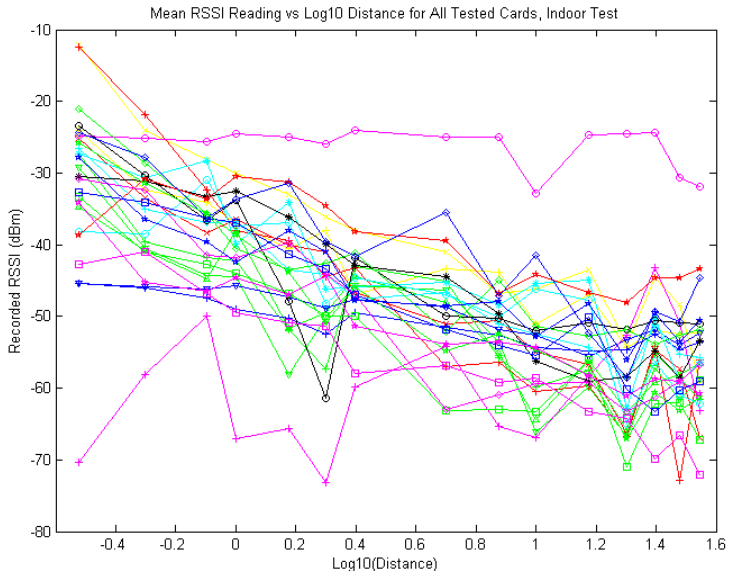
\includegraphics[width=\textwidth]{images/luiRSSI.png}
  \caption{Gemessener RSSI mit verschiedenen Access Points und Distanzen, aus \cite{lui2011differences}.}
  \label{fig:luiRSSI}
\end{figure}

\section{LANDMARC}
\label{ch:Vorherige:sec:LANDMARC}
Ni et al. stellen ein Ortungssystem auf Basis von Radio Frequency Identification (RFID) vor \cite{ni2004landmarc}.
Dazu werden aktive RFID-Tags als mobile Einheiten eingesetzt, diese sind mit einer Batterie ausgestattet und senden regelmäßig ihre gespeicherte ID aus.\\
Der Knoten ist mit einem Lesegerät (RFID-Reader) ausgestattet und empfängt die ID, der Knoten liefert dann die ID und ein Signalstärkelevel zwischen 1 und 8 zurück. 
Da das Signalstärkelevel nur eine sehr grobe Auflösung hat verbessern Ni et al. die Genauigkeit durch das Ausbringen von zusätzlichen Tags an bekannten, fixen Positionen, für die Bereichsortung ist dies aber nicht notwendig.\\
Die Autoren geben für ein Sendeintervall von 7,5 Sekunden eine Batterielaufzeit von 3-5 Jahren an, dabei sind die Tags klein genug und könnten, wie in der Einleitung gefordert, an einem Band um den Hals getragen werden.
%"System lässt sich leicht auf Bluetooth übertragen"

\section{Bluetooth}
\label{ch:Vorherige:sec:Bluetooth}
Hier habe ich noch kein Paper, es kommt aber fix noch mindestens ein System auf Bluetooth-Basis + Kritik an verschiedenen Buetooth Parametern.

\section{Time-of-flight Lokalisierung}
\label{ch:Vorherige:sec:TOF}
Aufgrund der Schwächen von RSS-basierten Systemen wurde auch über solche nachgedacht, die stattdessen oder zusätzlich die time-of-flight (TOF) messen, ein Beispiel für ein solches zeigen Wibowo et al. \cite{wibowo2009time}. 
Sie fordern optimalerweise Zugriff auf die physische Schicht (PHY) des 802.11 Protokolls, da auf dieseń aber üblicherweise kein Zugriff besteht messen sie TOF in der darüber liegenden MAC-Schicht.\\
Ein Knoten sendet einen Beacon Frame aus und protokollieren die Sendezeit, die mobile Einheit empfängt den Beacon Frame, protokolliert die Empfangszeit und die Sendezeit der gesendeten Antwort, der Knoten sichert die Empfangszeit der Antwort.
Nun sendet die mobile Einheit die zwei gespeicherten Zeitstempel an den Knoten, der mit diesen die Verarbeitungszeit auf der mobilen Einheit berechnen kann um dann die Distanz $d = c*(\frac{t_{empfangen} - t_{gesendet} - t_{Verarbeitung}}{2})$ zur mobilen Einheit zu bestimmen.
Dieses Schema lässt sich leicht von einer Fernlokalisierung in eine Selbstlokalisierung umwandeln indem man den Initiator des Vorgangs tauscht.\\
Die Notwendigkeit die Zeitstempel bereits in der PHY- beziehungsweise MAC-Schicht zu setzen erfordert Zugriff auf die Software des als Knoten verwendeten Access Points. 
Außerdem müssen die Zeitstempel im Bereich von Nanosekunden gesetzt werden und die Verarbeitungszeit vor/nach dem setzen muss sehr konstant sein, da eine Abweichung von $100ns$ bei $c = 299.792.458m/s$ bereits einen Fehler von $30m$ verursacht.\\
Muthukrishnan et al. beschreiben diese Problematik bei dem Versuch TOF ohne Zugriff auf die Software des APs umzusetzen \cite{muthukrishnan2006using}.
Sie kommen zu dem Ergebnis, dass sich die in der Spezifikation eingebauten Zeitstempelfunktionen wie das Network Time Protocol (NTP), Ping und die Zeitstempel in Beacon Frames nicht eignen, da sie zum einen nur eine Auflösung im Millisekundenbereich bieten und zum anderen von der Blockierungskontrolle von 802.11 (CSMA/CA) abhängen.

\subsection{Ultraschall}
Skibiniewski et al. nutzen Ultraschall für eine Fernlokalisierung mit TOF \cite{skibniewski2009simulation}.
Ultraschall kann nicht von WLAN APs empfangen werden und es muss zusätzliche Hardware installiert werden, das System soll hier dennoch Beachtung finden, da es für die Ortung von Baumaterial auf Baustellen entwickelt wurde.\\
Bei diesem System sendet zunächst der Knoten einen Beacon Frame der ZigBee Spezifikation (802.15.4) an die mobile Einheit, diese antwortet und sendet unmittelbar danach das Ultraschallsignal.
Das schnelle 2.4GHz ZigBee Signal dient dem Knoten dann als Referenz für den Sendezeitpunkt des Ultraschallsignals, welches wegen seiner langsamen Ausbreitungsgeschwindigkeit $c \approx 343m/s$ wesentlich weniger anfällig für ungenaue Zeitstempel ist. 
Außerdem kann die Zeit zwischen dem Aussenden des Beacon Frames und der Antwort gemessen werden um zusätzliche TOF-Informationen zu gewinnen. \\
Statt ZigBee ließe sich auch WLAN nutzen, ZigBee ist jedoch bereits auf niedrigen Energieverbrauch ausgelegt und wegen des Ultraschalls wäre trotzdem ein extra Knoten nötig.
Problematisch an der Lösung ist entweder der Energieverbrauch der Ultraschalleinheit oder die Reichweite, ausreichend kleine Einheiten reichen keine 100m weit und leiden trotzdem unter kurzer Batterielaufzeit.
Die Autoren schließen deshalb, dass noch Innovation in diesem Bereich notwendig ist um dieses System praktikabel zu machen.

\section{Ortung ohne mobile Einheit}
Eine Ortung ohne mobile Einheit erfüllt wegen ihrer Abwesenheit offensichtlich jede Anforderung an die Batterielaufzeit der mobilen Einheit.
Mit MonoPHY stellen Abdel-Nasser et al. ein System zur Ortung ohne mobile Einheit vor \cite{abdel2013monophy}. \\
Dazu verwenden sie einen 802.11n-fähigen Laptop und Access Point und analysieren die Channel State Information (CSI) der physischen Schicht (PHY) der zwischen AP und Laptop übertragenen Daten.
Um die bestehende Struktur von APs zu nutzen sollte das System angepasst und die CSI zwischen den APs gemessen werden.
Das System hat jedoch einige Aspekte, die es ungeeignet für die Aufgabenstellung machen.\\
Das System unterscheidet nicht zwischen Personen, sondern erkennt nur, dass jemand anwesend ist, außerdem ist es nur für eine Person in einem $100m^2$ gestaltet worden und müsste auf Baustellengröße und die Verfolgung mehrerer dutzend Personen erweitert werden.
Aber auch dann ist fraglich, wie gesichert werden kann, dass alle Personen durchgehend erkannt werden können, zum Beispiel wenn sich mehrere Personen auf oder in einem Transportfahrzeug aufhalten.
Auch ist es ohne Identifikation schwerer Fehler zu erkennen, wird fälschlicherweise angezeigt, dass sich noch eine Peron im Tunnel befindet kann oft durch ausrufen des Betreffenden festgestellt werden, dass dieser nicht im Tunnel ist. 
Hat man dagegen nur die Information, dass sich noch eine Person im Tunnel befindet müsste jede Gruppe durchgezählt werden und selbst dann bestünde die Möglichkeit, dass eine Person ohne das Wissen anderer in den Tunnel gegangen ist und diesen nicht mehr verlassen hat.\\
Weitere Probleme entstehen durch die Baumaschinen und Container, diese haben einen starken Einfluss auf die CSI und verdecken dadurch möglicherweise nahe Personen und die Fahrzeugführer.
Deshalb müssten diese Objekte ebenfalls als Entitäten angezeigt werden, die Anzeige diverser Kommandostände, Pausenräume und stehen gelassener Baumaschinen verwirrt im Notfall jedoch, da sich in jedem Objekt potentiell eine Person befinden könnte.\\
Die Veröffentlichung beruht außerdem auf der Verfügbarkeit der CSI, diese sind dort durch die Auswahl einer bestimmten Netzwerkkarte gegeben und sind nicht zwingend in einer bestehenden Struktur von APs verfügbar.
Als letzter Kritikpunkt steht die Verwendung eine offline-Phase, die, wie bereits diskutiert, wirtschaftlich nicht umsetzbar ist. \\ 
Somit erfüllt die Ortung ohne mobile Einheit zwar die Anforderungen an den Energieverbrauch, jedoch nicht die Forderung nach sicherer Erkennung von Abschnittswechseln, deshalb scheidet diese Technik zumindestens für Baustellen aus.


